\section{Motivating Application: \textit{Switching Linear System}}
\label{sec:motiviational_application}

In the following discussion, we present an example to motivate and lay
the foundation for the use of MoE in the control design problem. 
%
In particular, we propose a data-driven technique to automatically seek
switching controllers for multi-modal systems.
%  
Suppose we have two linear systems of the form 
\begin{equation}
    \begin{gathered}
        \dot{x} = A_1x = \bmat{0 & -1 \\ 2 & 0}x, \\
        \dot{x} = A_2x = \bmat{0 & -2 \\ 1 & 0}x,
    \end{gathered}
    \label{eq:unstable_closedloop}
\end{equation}
\noindent where each system is marginally stable as shown in
Figure~\ref{marginally_stable}.
%
Although the individual systems are not asymptotically stable, it is possible to
find a state-dependent switching rule that makes the resulting switched system
stable\cite{liberzon2003switching} (Figure~\ref{stable_switching}). 
%
We aim to learn a gating network $\mathbf{P}(x|\psi)$ to automatically divide
the state space into partitions and identify which of the two systems to execute
in each state partition, with the goal of asymptotically stabilizing the origin.
%
\begin{figure}[tb]
    \centering
    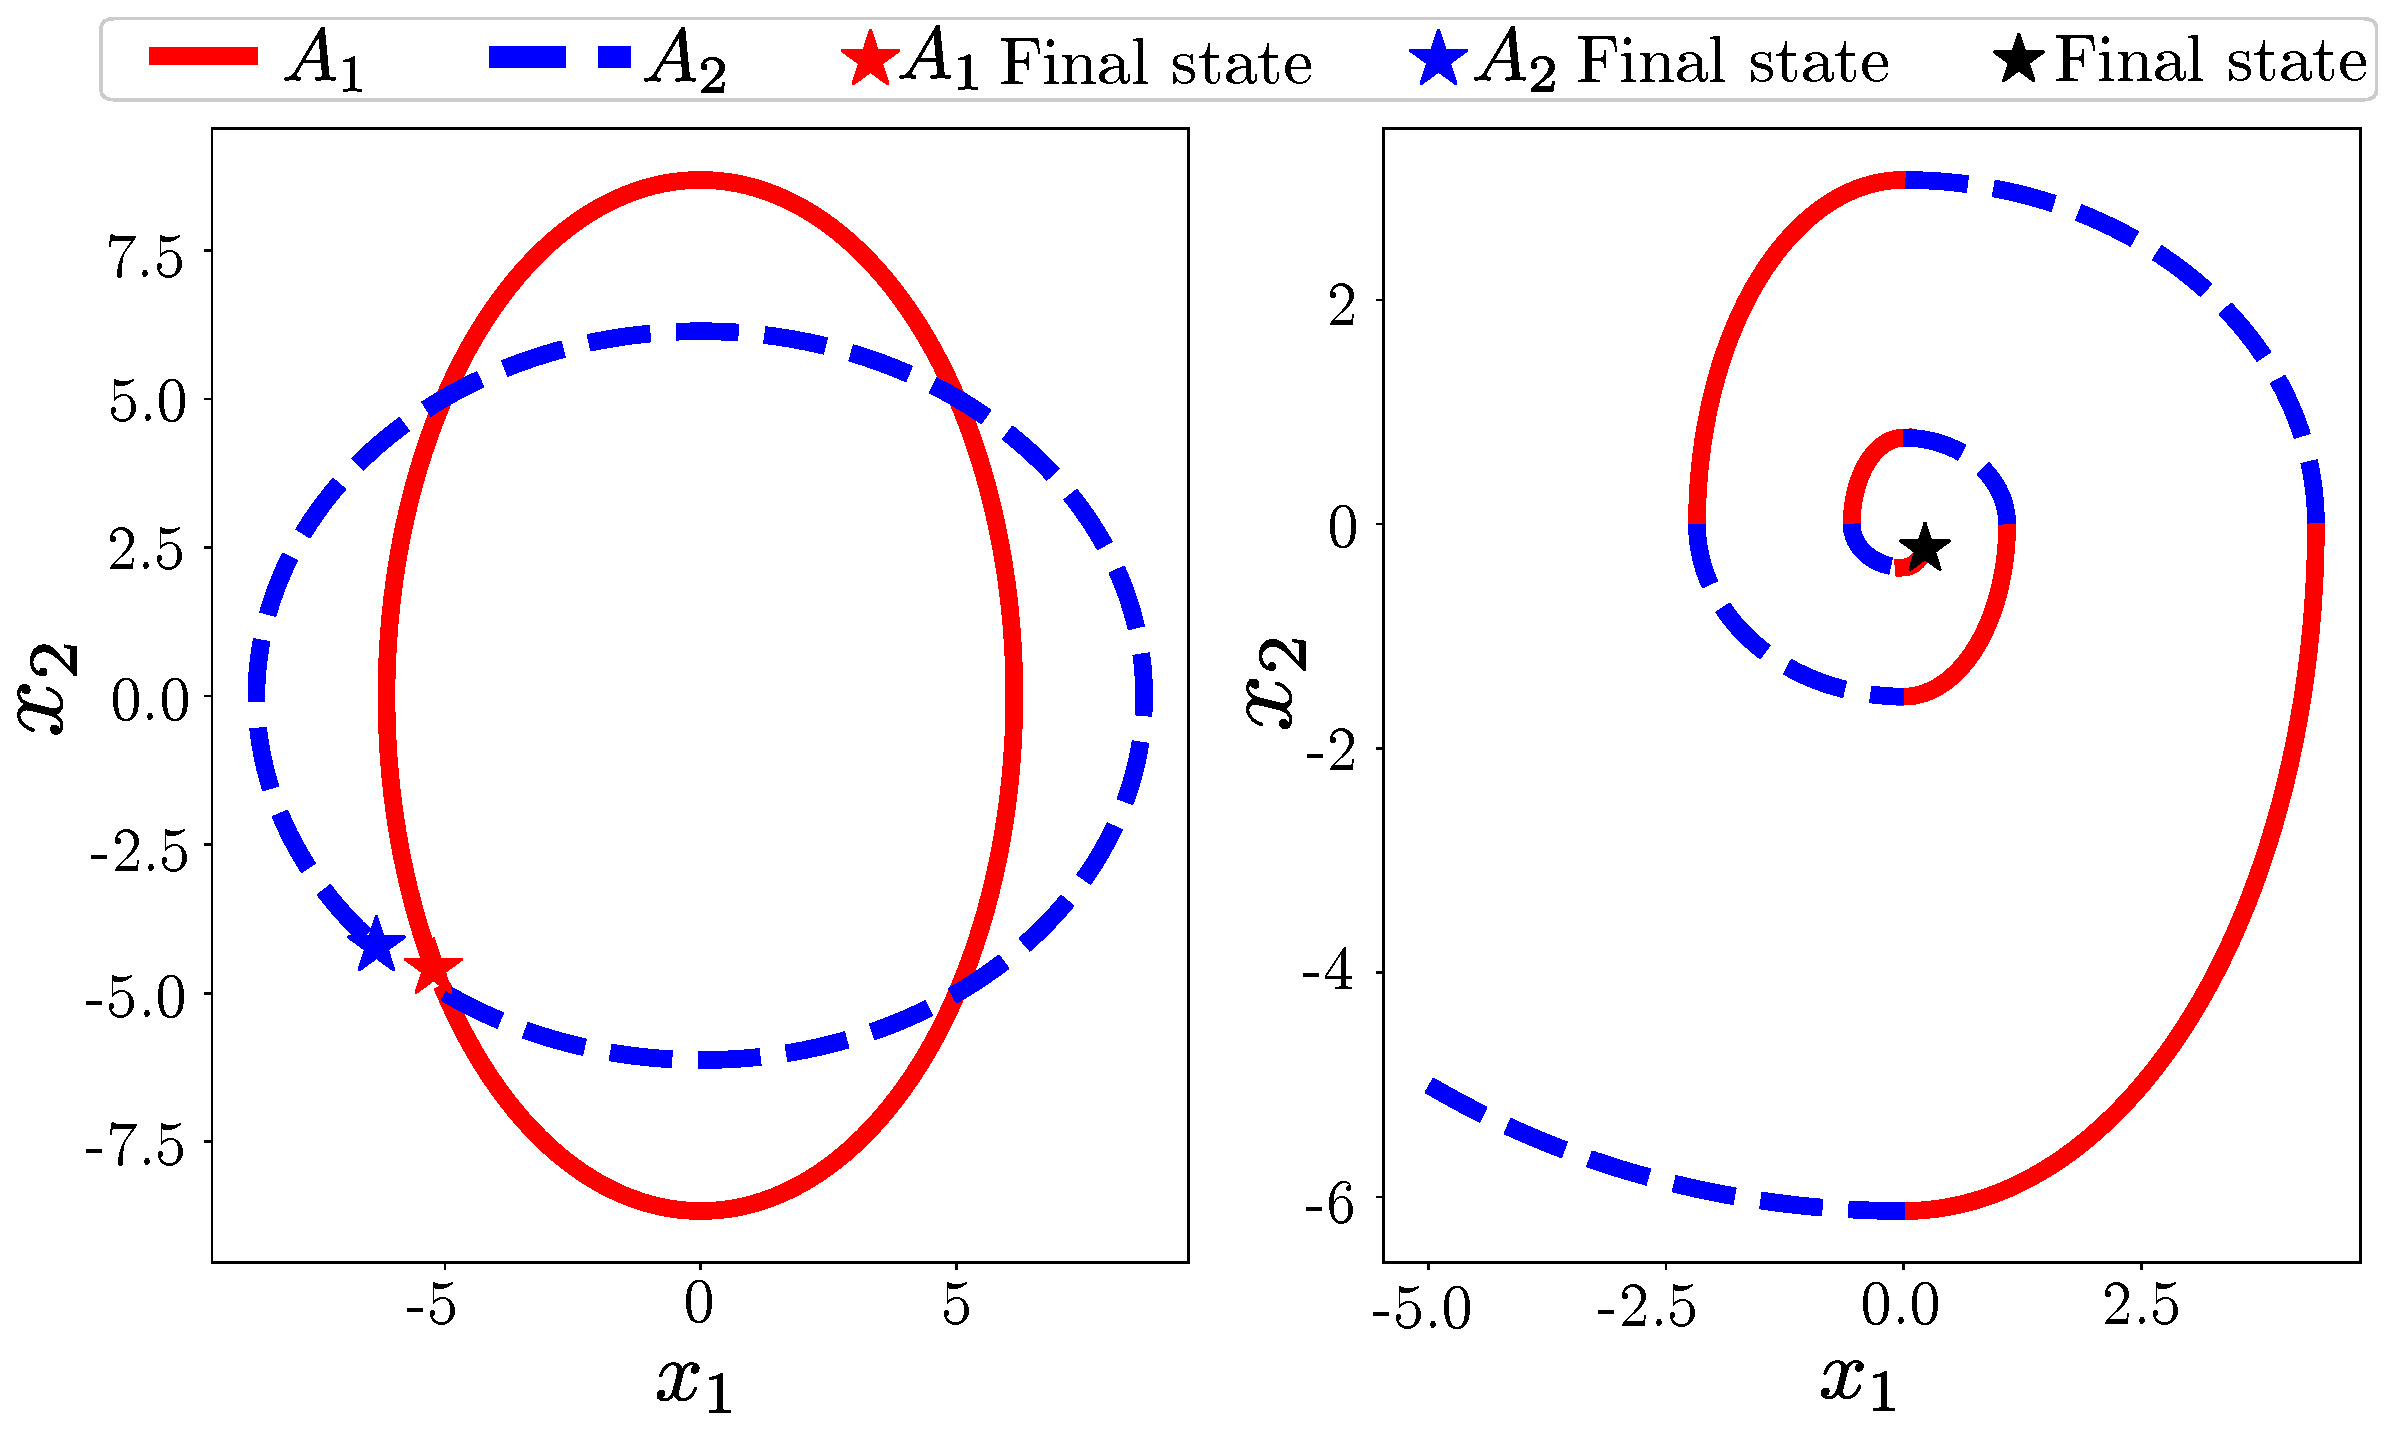
\includegraphics[width=0.7\linewidth]{switching_linear.eps}
    \subfloat[\label{marginally_stable}Two marginally stable closed-loop systems]{\hspace{0.5\linewidth}}
    \subfloat[\label{stable_switching}Asymptotically stable switching]{\hspace{0.5\linewidth}}
    \caption{Stable switching between two marginally stable systems }
    \label{fig:stableSwitching}
\end{figure}

Akin to the regression problem in Section~\ref{ssec:mixture_of_experts}, the
training dataset consists of \textit{input state-label} pairs, where the labels are
the performances of the trajectories generated under the current control law.
% 
In the case of the switching-control problem, we generate a trajectory and the
corresponding performance metric (labels) as follows.
%
Starting from some initial state $x(t=0)$, we sample a state partition index $i$
from the categorical distribution, whose probabilities are provided by the
gating network:
\begin{align*}
    i  \sim \text{Categorical} (\mathbf{P}(x(t)| \psi)).
\end{align*} 
Given the partition index $i$, the expert (control law) is given by a sample
from the Bernoulli probability distribution
\begin{align}
    F_i(\theta_i) = \begin{cases}
       0, & \theta_i > \frac{1}{2}, \\
       1, & \theta_i \leq \frac{1}{2},
    \end{cases}
    \label{eq:bernoulli}
\end{align}
\noindent where $F_i = 0$ corresponds to the first dynamics $\dot{x} = A_1 x$
and $F_i=1$ corresponds to $\dot{x} = A_2x$. The parameter $\theta_i$ of the
expert is to be learned, and it determines which of the two experts to
execute in each partition.
%
In order to ensure that the parameter $\theta_i$ of the expert serves as the
probability of the Bernoulli distribution, we use the \textsc{Sigmoid}
function\cite{sharma2017activation} to limit $\theta_i$ between 0 and 1.
%
The next state $x(t+\Delta t)$ in the trajectory is obtained from the following
integration scheme:
\begin{align*}
    x(t + \Delta t) = (1-F_i) A_1 x(t) + F_i A_2 x(t).
\end{align*}
%
We repeat this process to generate a trajectory for the time-horizon $T$.
%
The performance of the trajectory generated under the current parameters $(\psi,
\theta)$ can be quantified by the metric $\ell$ as
\begin{align*}
    \ell(x(t + \Delta t)) := \frac{1}{2} \norm{x(t + \Delta t)}{}^2.
\end{align*}
In Section~\ref{ssec:performance_objective}, we generalize the performance
metrics to be applicable to various dynamical systems and discuss how we can
encode desired characteristics of the controller.
%
From the performance metric $\ell$, we can construct the cost function
$\mathbb{L}$ similar to the standard MoE framework
in~\eqref{eq:log_normal_likelihood} as
\begin{align*}
    \mathbb{L} \Bigl(\{x(0), \dots, x(T)\} \Bigr)= \sum_{t=0}^{T} \sum_{i=1}^{N_F} \ell_i \Bigl(x_i(t + \Delta t) \Bigr) \; P_i \Bigl(x(t), \psi \Bigr) .
\end{align*}
\noindent In the upcoming sections, we generalize the MoE control-search
problem and provide techniques to efficiently learn the optimal decision
parameters from appropriate cost functions.


\section{Mixture of Expert Controller}
\label{sec:moe_methods}

Based on the motivating example provided in
Section~\ref{sec:motiviational_application}, we present a generalized
data-driven control design framework for hybrid dynamical systems.
%
In this framework, the controller is given by deep-net mixture of experts
$F(x;\theta)$, and the control switching scheme is governed by the gating
network $\mathbf{P}(x|\psi)$.
%
This technique allows us to observe the effects of mode changes from the
closed-loop trajectories and learn a switching mechanism to best control the
hybrid system across modes.
%
The objective is to learn the parameters $\theta_i$ of each expert and the
gating network $\psi$ that can achieve the desired performance.


%
Let $\phi(x_0, u, T)$ denote a closed-loop trajectory generated from a hybrid
dynamical model starting from initial state $x_0$.
%
We represent the dynamics of a hybrid system with the differential
inclusions\cite{goebel2009hybrid}
\begin{equation}
    \begin{cases}
        \dot{x} \in f(x, u), & x \in C,\\
        x^+ \in g(x, u), & x \in D,
    \end{cases}
    \label{eq:cont_and_guards}
\end{equation}
\noindent where $x \in \mathbb{R}^m$ is the state vector, and $u \in
\mathbb{R}^n$ is the input.
%
The set-valued mappings $f: \mathbb{R}^m \times \mathbb{R}^n \rightarrow
\mathbb{R}^m$ and $g: \mathbb{R}^m \times \mathbb{R}^n \rightarrow \mathbb{R}^m$
denote the flow and jump maps, respectively, where $C$ and $D$ are subsets of
$\mathbb{R}^m$ consisting of the feasible states under the flow and jump
rules, respectively. 
%
The notation $x^+$ indicates the state resulted by the jump rule $g$.
%


For every state $x$ in a trajectory, the control law first samples state
partition index $i$ from a categorical distribution and evaluates the
corresponding expert as
\begin{align}
    u(x; \psi, \theta) = \{F_i&(x; \theta_i) \; | \; i  \sim \text{Categorical} (\mathbf{P}(x| \psi)) \}.
    \label{eq:categorical}
\end{align} 
%
We use the metric $\ell : \mathcal{X} \times \mathcal{U} \rightarrow
\mathbb{R}$ to measure the performance of the sampled experts, which we discuss
in depth in Section~\ref{ssec:performance_objective}.
%
% The running cost plays the role of \it{prediction error} \normalfont in the
% construction of the cost function $\mathcal{L}$ as shown
% in~\eqref{eq:original_normal_likelihood}.
%
The goal is to learn the decision parameters $(\psi, \theta)$ that minimize the
metric $\ell$ for all initial states in the state space.
%
We pose the search over the parameters of the experts and the gating network as the following optimization problem.
\begin{equation}
    \begin{aligned}
        \underset{\psi, \theta}{\textrm{minimize}} 
        & & &\int_0^T \ell (x(t),u) \dd t , \\%
        \textrm{subject to}
        & & &\begin{cases}
                    \dot{x} \in f(x, u), & x \in C,\\
                    x^+ \in g(x, u), & x \in D,
                \end{cases}\\%
        & & u = \{F_i&(x; \theta_i) \; | \; i  \sim \text{Categorical} (\mathbf{P}(x| \psi)) \}.
    \end{aligned}
    \label{eq:moe_opt}
\end{equation}
%
In Section~\ref{ssec:training_moe}, we provide a procedure to solve the
optimization problem~\eqref{eq:moe_opt} via stochastic gradient descent. 
\begin{rem}
    Without prior knowledge injected to the gating network, the samples from the
    categorical distribution in~\eqref{eq:categorical} initially explore the
    performance of most, if not all, of the expert controllers.
    %
    As the parameters converge to their optimal values, the samples from the
    categorical distribution correspond to the indices of the single best
    experts and the control law in~\eqref{eq:categorical} is equivalent
    to~\eqref{eq:best_expert_prediction}.
\end{rem}

\subsection{Performance Objective}
\label{ssec:performance_objective}
%
We present two viable choices for the running cost function. 
\begin{enumerate}
    \item \textbf{Accumulated loss}: is the total quadratic loss between the desired
    state $x^*$ and the states generated under the current control law. We also
    incur a cost on the control authority as follows.
    \begin{equation}
        \begin{gathered}
            \ell(x, u) = \frac{1}{2}(x - x^*)^\top \mathcal{Q} (x - x^*) + \frac{1}{2} u^\top \mathcal{R} u , 
            % \ell(\phi, u) = \int_0^{T}  \ell(x(t), u)\dd t,
        \end{gathered}
    \label{eq:accumulatedLoss}
    \end{equation}
    \noindent where $\mathcal{Q} \succ 0$ denotes a positive definite matrix and
    $\mathcal{R} \succeq 0$ represents a positive semi-definite matrix.
    %
    This construction encourages trajectories to reach the desired equilibrium
    with minimum effort and shortest time.
    %

    We modify the likelihood function $\mathbb{L}$ constructed
    in~\eqref{eq:log_normal_likelihood} to incorporate the accumulated loss
    $\ell(x, u)$.
    %
    The quadratic loss in~\eqref{eq:accumulatedLoss} plays the role of prediction
    error in the likelihood function.
    %
    Similar to the regression problem provided in
    Section~\ref{ssec:mixture_of_experts}, we want the likelihood to be maximum
    when the running cost incurred by expert $i$ is low and the responsibility
    of the expert is high.
    %
    We can obtain this characteristics by designing the likelihood as
    \begin{align}
        \mathbb{L}(\phi) = \sum_{t=0}^{T} \sum_{i=1}^{N_F} - \ell \Bigl(x(t+\Delta t), F_i \Bigr) P_i\Bigl(x(t) | \psi \Bigr)  .
        \label{eq:accumulated_likelihood}
    \end{align}
    %
    Algorithm~\ref{algo:accumulated_loss} outlines how we construct the
    likelihood from a trajectory.
    %
    In this procedure we check the performance of each expert at every
    integration step.
    %
    To do so, starting at initial state $x_0$, we integrate the dynamics
    in~\eqref{eq:hybrid_dynamics} for one time step $\Delta t$ using all the
    experts in $F(x_0;\theta)$.
    %
    We retrieve all the states $\{ x_i(\Delta t) , i \in \{1, \dots N_F \}\}$
    obtained from the integration and evaluate the running cost $\ell(x_i(\Delta
    t), F_i)$ incurred by each expert.
    %
    Each running cost $\ell(x_i(\Delta t), F_i)$ is weighed by its
    \textit{responsibility} $P_i(x_0 | \psi)$ and summed across experts to get
    the likelihood.
    \begin{algorithm}[tb]
        \setstretch{1.2}
        \caption{Accumulated Loss}
        \label{algo:accumulated_loss}
        \small
        \hspace*{\algorithmicindent} \textbf{Input}: $x_0, \theta, \psi$
        \begin{algorithmic}[1]
            \State $\mathbb{L} \leftarrow 0$
            % \algrenewcommand\algorithmicindent{0em} % No indent
                \For{$t = 0:\Delta t:T$}     
                \For{$j=1:N_F$}\Comment{Evaluate performance of each expert}
                    \State $x_j(t+\Delta t) \leftarrow \texttt{Moreau's one time step}(x(t), F_j(x(t), \theta_j))$\Comment{Algorithm~\eqref{algo:moreau}}
                    \State $\mathbb{L} \leftarrow \mathbb{L} - \ell(x_j(t+\Delta t), F_j) \; P_j(x(t) | \psi)$
                \EndFor
                \State $i \sim \text{Categorical}\Bigl(\mathbf{P}(x(t)| \psi)\Bigr)$ \Comment{Sample a bin number}
                \State $x(t + \Delta t) \leftarrow \texttt{Moreau's one time step}(x(t), F_i(x(t), \theta_i))$
                \EndFor
            \State \textbf{return} $\mathbb{L}$
        \end{algorithmic}
    \end{algorithm}
    %
    Notice that by checking the running cost of each expert for every state, the
    computation of the likelihood is prone to the curse of dimensionality.
    %
    We minimize the amount of computation needed to compose the likelihood by
    selecting one state from the collection $\{ x_i(\Delta t) , i \in \{1,
    \dots N_F \}\}$ to continue the integration.
    %
    We select the expert responsible for generating the next state $x(\Delta t)$ from the
    categorical distribution~\eqref{eq:gating_categorical}.
    %
    This process is repeated for every time step in the trajectory.
    % Notice that for each state $x(t)$, we need to test the performance of each expert. 
    % %
    % For instance, if there are $100$ states in a trajectory and $3$ experts, we need to evaluate $\ell$ $300$ times.

  
    \item \textbf{Minimum trajectory loss (MTL)}: In some cases,
    accumulated loss may not reflect the desired behavior of the dynamical
    systems.
    %
    For instance, suppose we want to swing-up the simple pendulum to the upright
    equilibrium. 
    %
    For an underactuated pendulum, the controller needs to swing about the
    downward equilibrium, moving the states closer and further away from the
    upright.
    %
    Accumulated loss incurs a lot of cost in such scenarios and the control
    search would get stuck in local minima.
    %
    In such cases, a successful loss function encourages trajectories that
    \it{eventually} \normalfont lead to a minimum cost.
    %
    Hence, we construct the minimum trajectory loss (MTL), which is composed of
    the lowest cost incurred across the entire trajectory and the
    responsibilities of the experts that led to the minimum cost.
    %
    The resulting likelihood $\mathbb{L}$ is given by
    \begin{equation}
        \begin{gathered}
            t_{min} = \underset{t}{\textrm{inf}} \; \{ \ell(x(t), u): x(t) \in \phi(x_0, u, T) \}  \\
            \mathbb{L}(\phi) = - \frac{\ell(x(t_{min}), u)}{C} \sum_{t=0}^{t_{min}}P_i(x(t) | \psi) 
        \end{gathered} 
    \end{equation}
    \noindent where $C > 0$ is a normalization factor.
    %
    Unlike accumulated loss, MTL does not particularly reward low effort or
    short time trajectories, but it equally rewards two trajectories
    as long as they both reach the desired state within the time horizon $T$. 
    %
    Moreover, MTL does not need to evaluate the performance of each expert at
    every integration step, as shown in Algorithm~\eqref{algo:mtl}; this greatly
    reduces the computational cost.
    %
    \begin{algorithm}[tb]
        \setstretch{1.2}
        \caption{Minimum Trajectory Loss}
        \label{algo:mtl}
        \small
        \hspace*{\algorithmicindent} \textbf{Input}: $x_0, \theta, \psi$
        \begin{algorithmic}[1]
            % \algrenewcommand\algorithmicindent{0em} % No indent
            \State $\phi \leftarrow \{ x_0 \}$
                \For{$t = 0:\Delta t:T$}     
                    \State $i \sim \text{Categorical}\Bigl(\mathbf{P}(x(t)| \psi)\Bigr)$ \Comment{Sample a bin number}
                    \State $x(t + \Delta t) \leftarrow \texttt{Moreau's one time step}(x(t), F_i(x(t), \theta_i))$\Comment{Algorithm~\eqref{algo:moreau}}
                    \State $\phi \leftarrow \phi \cup x(t+\Delta t)$
                \EndFor
                \State $t_{min} = \underset{t}{\textrm{inf}} \; \{ \ell(x(t), u): x(t) \in \phi\}$
                \State $\mathbb{L} = - \ell(x(t_{min}), u) \sum_{t=0}^{t_{min}}P_i(x(t) | \psi)  $
            \State \textbf{return} $\mathbb{L}$
        \end{algorithmic}
    \end{algorithm}
\end{enumerate}

\subsection{State Sampling}
\label{ssec:state_sampling}

We intend to find a solution to the optimization problem
in~\eqref{eq:moe_opt} for all initial states $x_0$ in the
state space.
%
To do so, we generate the running cost $\ell$ from \textit{a batch of initial
states} and update the parameters $(\psi, \theta)$ \textit{iteratively} via
stochastic gradient descent.
%
We need to collect the batch of initial states in an efficient manner.
%
It is computationally expensive to merely discretize the vast state
space into batches of initial states. 
%
To efficiently sample the initial states, we use a combination of greedy and
explorative state sampling techniques.
%
Greedy state sampling, commonly known as \textsc{DAgger}, is a technique
adapted from imitation learning~\cite{ross2011no}.
%
This method collects states most visited under the current parameters $(\psi,
\theta)$ and concentrates on refining the performance of the controller on these
states.
%
For instance, suppose we are solving the optimization in~\eqref{eq:moe_opt} to
obtain a controller that swings up an underactuated simple pendulum to the
upright.
% %
Initially, the parameters $(\psi, \theta)$ may result in a controller that swings the
pendulum to the downward equilibrium irrespective of where it started.
%
Thus, it is most efficient to first expose the training to the cost incurred by
visiting the downward equilibrium.
%
In this technique, we first sample several initial states randomly and generate
trajectories using the current parameters.
%
Then, we randomly select $N_d$ samples from the states visited in the trajectory. 
%
At first, the $N_d$ samples mostly consist of states near the downward equilibrium.
%
As the parameter update continues, \textsc{DAgger} starts sampling states that
are closer to the upright equilibrium.
%
This efficient state exposition is pivotal for the convergence to the optimal
parameters.



The explorative state sampling technique exposes the training to the rewards of approaching and 
remaining close to $x^*$.
%
It also uses random sampling to explore new control strategies and recover from locally optimal
solutions.  
%
This method collects $N_r$ initial states around the neighborhood of the desired
equilibrium by drawing samples from the normal distribution $x_0 \sim \mathcal{N}(x^*, \delta)$,
whose mean is $x^*$ and the standard deviation is a small constant $\delta$.
%
The combination of greedy and explorative state sampling techniques helps to
quickly refine the performance of the current controller and converge to the desired behavior.
%
In a single batch training, we compute the running cost as an expectation
over $N_{\mathcal{D}} = N_d+N_r$ samples as follows:
\begin{align*}
    J(\phi, u) = \mathbb{E}_{x_0 \in \mathcal{D}_N}[ \mathbb{L}(\phi(x_0, u, T))]
\end{align*}
\noindent where $\mathcal{D}_N$ is a collection of $N_{\mathcal{D}}$ initial state samples.

\subsection{Training Mixture of Expert Controller}
\label{ssec:training_moe}

%
We solve the optimization problem in~\eqref{eq:moe_opt} following the procedure
outlined in Algorithm~\eqref{algo:moe_training}.
%
At the beginning of the training, we add a batch of initial states $x_0$ to the
collection $\mathcal{D}_N$. These initial states are obtained from the greedy
and explorative state sampling techniques. 
%
For every initial state in the batch, we generate a trajectory for time horizon $T$.
%
The running cost of these trajectories are given by the accumulated cost
(Algorithm~\eqref{algo:accumulated_loss}) or minimum trajectory loss
(Algorithm~\eqref{algo:mtl}), depending on the desired closed-loop behavior. 
%
We average the running cost of each of the trajectories and perform
\textit{expectation maximization} with respect to the decision parameters
$(\psi, \theta)$.
%
We invoke a variant of stochastic gradient descent known as
\textsc{Adam}~\cite{kingma2014adam} to efficiently train the parameters with
adaptive learning rates $\alpha_i$.
%
We leverage auto-differentiation techniques to back-propagate on the gradient of
the likelihood with respect to the learned parameters.
%
In particular, we use forward-mode auto-differentiation~\cite{revels2016forward}
to take the gradient through the trajectory generated from Moreau's integration
scheme.
%
Although not explored in this work, it is possible to design adjoint methods for
hybrid systems to efficiently back-propagate on the likelihood through
reverse-mode auto-differentiation techniques.
%
\begin{algorithm}[tb]
    \setstretch{1.2}
      \caption{Solution to the Optimization Problem~\eqref{eq:moe_opt}}
      \label{algo:moe_training}
      \small
      \begin{algorithmic}[1]
          \algrenewcommand\algorithmicindent{0em} % No indent
          \State $\mathcal{D}_N \gets \{x_0\}_{(N_{\mathcal{D}})}$  \Comment{$N_{\mathcal{D}}$ initial state samples} 
          \algrenewcommand\algorithmicindent{1.1em} % Change indent back to default
          \While{$i < $ \texttt{maximum iteration}}
          \State $J \gets 0$\Comment{Batch loss}
          \For{$x_0 \in \mathcal {D}_N$}
              \State $\mathbb{L}$ = \texttt{Performance objective}($x_0, \psi, \theta$) \Comment{Algorithm~\eqref{algo:accumulated_loss} or~\eqref{algo:mtl}}
              \State $J \gets J + \mathbb{L}/N_{\mathcal{D}}$ 
          \EndFor
          \State $\theta \gets \theta + \alpha_i \nicefrac{\partial J}{\partial \theta}$\Comment{SGD step}
          \State $\psi \gets \psi + \alpha_i \nicefrac{\partial J}{\partial \psi}$
          \State $\mathcal{D}_N \gets \{x_0\}_{(N_{\mathcal{D}})}$\Comment{New initial state samples}
          \State $i \;\:\gets i + 1$
          \EndWhile
          \State \textbf{return} $\theta$
      \end{algorithmic}
  \end{algorithm}

\subsection{Back-propagation through Hybrid Dynamics}
\label{ssec:backprop_hybrid}

The training framework outlined~\eqref{eq:moe_opt} allows us to observe the
effects of contacts in the closed-loop trajectories and infer a controller that
either uses the contact to its advantage or minimizes its adverse effects.
%
In this section, we look at the relevant parts of the back-propagation to give
insight on how this is achieved.
%
We also show that despite the state jumps in the hybrid dynamics, the
derivatives involved in the back-propagation are well-defined.

Suppose we generate a short trajectory $\phi$ with the sampled expert control
parameter $\theta_i$.
%
Forward-mode auto-differentiation evaluates the gradient of the accumulated cost
with respect to $\theta_i$ as 
\begin{align*}
    \frac{\partial \ell}{\partial \theta_i} = \sum_{t=0}^{T} \frac{\partial \ell}{\partial x_t} \frac{\partial x_t}{\partial \theta_i} ,
\end{align*}
\noindent where $R=0$ for simplicity.
%
Without loss of generality, we take one integration step for the reminder of
this discussion. 
%
In that step, a contact event is triggered causing the velocities to jump
between the initial state $x_0$ and the following state $x_1$. 
%
Hence, we focus on 
\begin{align*}
    \frac{\partial \ell}{\partial \theta_i} = \frac{\partial \ell}{\partial x_1} \frac{\partial x_1}{\partial \theta_i},
\end{align*}
%
We can expand the gradient further as 
\begin{align*}
    \frac{\partial \ell}{\partial \theta_i} = \frac{\partial \ell}{\partial x_1} \Bigl( \frac{\partial x_1}{\partial u} \frac{\partial u}{\partial \theta_i} + \frac{\partial x_1}{\partial \lambda}\frac{\partial \lambda}{\partial \theta_i}\Bigr),
\end{align*}
\noindent where $\lambda$ holds the contact forces.
%
We can compute the first term from Moreau's integration step as
\begin{align*}
    \frac{\partial x_1}{\partial u} \frac{\partial u}{\partial \theta_i} = 
    \bmat{M^{-1}B \Delta t^2/2 \\ M^{-1}B \Delta t} \frac{\partial u}{\partial \theta_i},
\end{align*} 
%
At first glance, it may seem the derivative $\frac{\partial x_1}{\partial
\lambda}\frac{\partial \lambda}{\partial \theta_i}$ does not exist due to
the discontinuity in the states. 
%
A closer observation reveals that  $\frac{\partial x_1}{\partial \lambda}$
determines how the \it{post-impact velocity is affected by the
contact forces}.~\normalfont
%
In fact, the derivative can be found from Moreau's integration as 
\begin{align*}
    \frac{\partial x_1}{\partial \lambda} = \bmat{W_N & W_T }, 
\end{align*}
%
demonstrating that the gradient exists even if a state jump has occurred. 
%
This term is crucial in adjusting the decision parameters in response to how the
contact force assists or inhibits the system.
%
If the contact forces affect the \it{post-impact} \normalfont velocity such that
the resulting generalized coordinates are closer to the desired state $x^*$,
then the gradient $\frac{\partial \ell}{\partial x_1} \frac{\partial
x_1}{\partial \lambda}\frac{\partial \lambda}{\partial \theta_i}$ adjusts the
parameter $\theta_i$ to favor states undergoing contact events. 
%
Indeed, we demonstrate this behavior in simulation and real-world experiments in
Section~\ref{ssec:cartpole_with_walls}.
%
Conversely, if the contact forces move the states further away from $x^*$, the
gradient leads to control parameters that attempt to recover from the outcomes
of the contact events.
%
We also demonstrate this behavior on a walking robot example in
Section~\ref{sssec:rimless_wheel_model}.
